\let\negmedspace\undefined
\let\negthickspace\undefined
\documentclass[journal]{IEEEtran}
\usepackage[a5paper, margin=10mm, onecolumn]{geometry}
%\usepackage{lmodern} % Ensure lmodern is loaded for pdflatex
\usepackage{tfrupee} % Include tfrupee package

\setlength{\headheight}{1cm} % Set the height of the header box
\setlength{\headsep}{0mm}     % Set the distance between the header box and the top of the text

\usepackage{gvv-book}
\usepackage{gvv}
\usepackage{cite}
\usepackage{amsmath,amssymb,amsfonts,amsthm}
\usepackage{algorithmic}
\usepackage{graphicx}
\usepackage{textcomp}
\usepackage{xcolor}
\usepackage{txfonts}
\usepackage{listings}
\usepackage{enumitem}
\usepackage{mathtools}
\usepackage{gensymb}
\usepackage{comment}
\usepackage[breaklinks=true]{hyperref}
\usepackage{tkz-euclide} 
\usepackage{listings}
\def\inputGnumericTable{}                                 
\usepackage[latin1]{inputenc}                                
\usepackage{color}                                            
\usepackage{array}                                            
\usepackage{longtable}                                       
\usepackage{calc}                                             
\usepackage{multirow}                                         
\usepackage{hhline}                                           
\usepackage{ifthen}                                           
\usepackage{lscape}

\begin{document}

\bibliographystyle{IEEEtran}
\vspace{3cm}

\title{CHAPTER - 8\\Application of Integrals}
\author{EE24BTECH11061 - Rohith Sai}
{\let\newpage\relax\maketitle}

\renewcommand{\thefigure}{\theenumi}
\renewcommand{\thetable}{\theenumi}
\setlength{\intextsep}{10pt} % Space between text and floats

\numberwithin{figure}{enumi}
\renewcommand{\thetable}{\theenumi}

\section*{Exercise : 8.3 (Miscellaneous)}
\begin{enumerate}
\item [6)] Find the area enclosed between the parabola $y^2 = 4ax$ and the line $y = mx$.\\

\textbf{Solution (using the General Method):}\\
The given curves are the parabola $y^2 = 4ax$ and the line $y = mx$. To find the points of intersection, we represent the curves in the matrix form of a conic section.

The parabola $y^2 = 4ax$ can be written in matrix form as:
\begin{align}
y^\top V y + u^\top y + f = 0
\end{align}

where:
\begin{align}
V = \myvec{0 & 0 \\ 0 & 1}, \, u = \myvec{-2 \\ 0}, \, f = 0
\end{align}

The line $y = mx$ can be represented as:
\begin{align}
m^\top y + d = 0
\end{align}

where:
\begin{align}
m = \myvec{1 \\ -m}, \, d = 0 \\
\implies m = \myvec{1 \\ -1}
\end{align}

Using the matrix form for the intersection points:
\begin{align}
y_i &= h + k_i m
\end{align}

where:
\begin{align}
k_i &= \frac{-m^\top \brak{Vh + u} \pm \sqrt{\brak{m^\top \brak{Vh + u}}^2 - g\brak{h} m^\top V m}}{m^\top V m}
\end{align}

Here, $h$ is the center of the conic. Since it's a parabola, we take $h = \myvec{0 \\ 0}$.

Substitute the values:
\begin{align}
k_i &= \frac{-\myvec{1 & -1} \myvec{0 \\ -2} \pm \sqrt{\left(\myvec{1 & -1} \myvec{0 \\ -2}\right)^2}}{\myvec{1 & -1} \myvec{0 & 0 \\ 0 & 1} \myvec{1 \\ -1}}
\end{align}

Simplifying:
\begin{align}
k_i &= \frac{2 \pm \sqrt{4}}{1}
\end{align}

Thus:
\begin{align}
k_1 &= 4, \, k_2 = 0
\end{align}

Substitute back to find $y_i$:
\begin{align}
y_1 &= \myvec{0 \\ 0} + 4 \myvec{1 \\ -1} = \myvec{4 \\ 4}
\end{align}

\begin{align}
y_2 &= \myvec{0 \\ 0}
\end{align}

Therefore, the points of intersection are $(0, 0)$ and $(4, 4)$.

The enclosed area is the integral of the difference between the line and the parabola from $x = 0$ to $x = 4$:
\begin{align}
A &= \int_0^4 \brak{x - \sqrt{4x}} \, dx
\end{align}

\textbf{Solution (using the Trapezoidal Rule):}\\

The total area can be approximated by dividing the region into small trapezoidal strips and summing their areas:
\begin{align}
A &= \frac{1}{2} h \brak{y\brak{x_1} + y\brak{x_0}} + \frac{1}{2} h \brak{y\brak{x_2} + y\brak{x_1}} + \cdots + \frac{1}{2} h \brak{y\brak{x_n} + y\brak{x_{n-1}}}
\end{align}

Simplifying:
\begin{align}
A &= h \left[ \frac{1}{2} \brak{y\brak{x_0} + y\brak{x_n}} + y\brak{x_1} + \cdots + y\brak{x_{n-1}} \right]
\end{align}

Let $A\brak{x_n}$ be the area enclosed by the curve from $x = x_0$ to $x = x_n$, where $\brak{x_0, x_1, \dots, x_n}$ are equidistant points with step size $h$:
\begin{align}
A\brak{x_n + h} &= A\brak{x_n} + \frac{1}{2} h \brak{y\brak{x_n + h} + y\brak{x_n}}
\end{align}

Repeating this process until we reach the desired area and discretizing the steps, let $A\brak{x_n} = A_n$ and $y\brak{x_n} = y_n$:
\begin{align}
A_{n+1} &= A_n + h y_n + \frac{1}{2} h^2 y^{\prime}_n
\end{align}

In the given question:
\begin{align}
y_n &= \sqrt{4 - x_n^2} + x_n - 2
\end{align}
and:
\begin{align}
y^{\prime}_n &= \frac{-x_n}{\sqrt{4 - x_n^2}} + 1
\end{align}

Thus, the general difference equation becomes:
\begin{align}
A_{n+1} &= A_n + h \brak{\sqrt{4 - x_n^2} + x_n - 2} + \frac{1}{2} h^2 \brak{\frac{-x_n}{\sqrt{4 - x_n^2}} + 1}
\end{align}

\textbf{Final Result:}\\
Theoretical area: $\frac{8}{3} \approx 2.67$ sq. units.\\
Computed area using the trapezoidal rule: $2.658$ sq. units.

The plot showing the area enclosed between the parabola $y^2 = 4x$ and the line $y=x$ is shown below:
\begin{figure}[H]
    \centering
    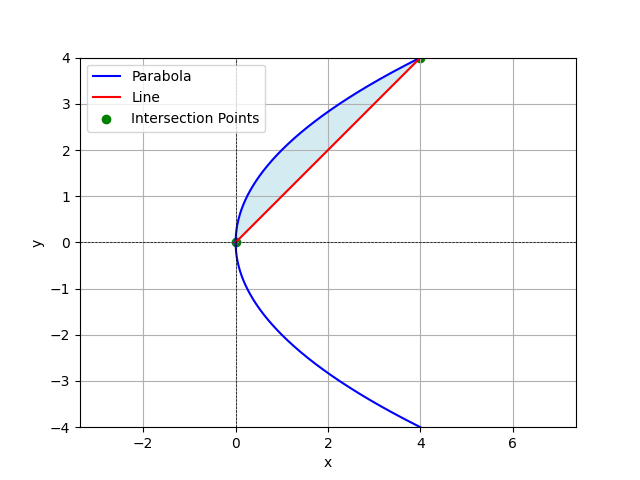
\includegraphics[width=\columnwidth]{figs/figure.png}
\end{figure}

\end{enumerate}
\end{document}
